\subsection{Limbisches System und Hippocampus} \label{subsec:limisches_system} \index{System! limbisches}
Der Begriff des limbischen Systems wurde zum ersten Mal 1878 durch den Neurologen Paul Broca geprägt. Er verwendete ihn, um die Gehirnstrukturen, die sich saumartig (limbisch) um den Balken und Thalamus herumziehen, zu definieren \textsuperscript{\cite[Kap.~18]{neurowissenschaften_baer}}. Dieser Begriff hat sich seitdem erweitert und steht nunmehr für die funktionelle Einheit, die für die Entstehung des Triebverhaltens und der Verarbeitung von Emotionen und Erinnerungen zuständig ist. Die dazugehörigen Zentren setzen sich aus allocorticalen und subcortikalen Bereichen zusammen, die dabei häufig eher ungenau definiert sind. Meistens werden dabei die Strukturen \textbf{Hippocampus}, \textbf{Gyrus cinguli}, \textbf{Gyrus parahippocampalis}, \textbf{Corpus amygdaloideum} (Amygdala) und \textbf{Corpus mammillare} \index{Corpus! mammillare} \index{Mammillarkörper} mit dem limbischen System in Verbindung gebracht \textsuperscript{\cite[Kap.~9]{trepel2011neuroanatomie}}.\\ 
\\ \noindent Ein Netzwerk, das dabei all diese Strukturen miteinander verbindet, ist der sogenannte \textbf{Papez-Neuronenkreis}. Der Hippocampus erhält den Großteil seiner Afferenzen über den Tractus perforans aus der Area entorhinales des Gyrus parahippocampalis. Anschließend verlassen Efferenzen den Hippocampus über den Fasertrakt des Fornix. Dieser endet in den Corpus mammillare des Hypothalamus. Über den Fasciculus mammillothalamicus wird dann weiter in den Ncl. anterior des Thalamus projiziert, der wiederum Fasern zum Gyrus cinguli sendet. Von dort gehen Fasern zur Area entorhinalis im Gyrus parahippocampalis, der dann zurück zum Hippocampus Projektionen sendet. Damit schließt sich der Neuronenkreis. Bei seiner Entdeckung im Jahre 1930 durch den Neurologen James Papez wurde zunächst vermutet, dass er essentiell an der Entstehung von Emotionen beteiligt ist. Nach heutigem Kenntnisstand dient er allerdings eher als wichtigste Grundlage zur Konsolidierung erlernter Gedächtnisinhalte aus dem Kurz- in das Langzeitgedächtnis \textsuperscript{\cite[Kap.~9]{trepel2011neuroanatomie}}. Im Folgenden werden einzelne wichtige Strukturen des limbischen System (Gyrus cinguli, Hippocampus und Amygdala) etwas ausführlich besprochen und anschließend wird dessen allgemeine Funktion zum aktuellen Forschungsstand erläutert.

\subsubsection*{Gyrus cinguli} \index{Gyrus! cinguli} \index{Cortex! cinguli}
Der \textbf{Gyrus cinguli} ist oberhalb des Corpus callosums lokalisiert und zusammen mit dem Hippocampus macht der den Großteil des limbischen Systems aus (Abb.~\ref{fig:cingulaerer_Cortex}). Seine Verbindung zu anderen Arealen, besonders zum Gyrus parahippocampalis, ist ein subcortikaler Fasertrakt, der als \textbf{Cingulum}\index{Cingulum} bezeichnet wird. Der cinguläre Cortex steht außerdem, neben bestimmten Strukturen des limbischen Systems, auch mit dem Assoziationscortex und dem Striatum in Verbindung. Aus diesem Grund wird ihm eine wichtige Rolle in der psycho- und lokomotorischen Dynamik zugeschrieben. Zusätzlich projiziert der Gyrus cinguli auch zum Ncl. facialis des Hirnstamms. Über diese Verbindung werden emotionale Gesichtsbewegungen, wie Lachen und Weinen, ausgelöst. Dabei wird der cinguläre Cortex auch durch die Amygdala gesteuert \textsuperscript{\cite[Kap.~9]{trepel2011neuroanatomie}}.

\begin{figure}[H]
    \centering
    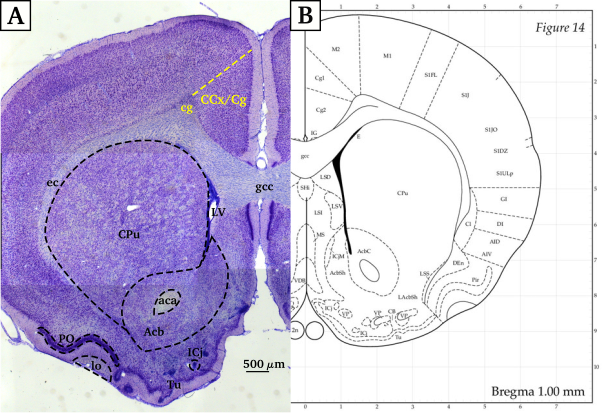
\includegraphics[width=0.9\textwidth]{pictures/Basalganglia/cingulaerer_Cortex.png}
    \caption[Gyrus cinguli]{\textbf{Gyrus cinguli.} \textbf{A:} Der Gyrus cinguli (CCx/Cg) liegt oberhalb des Corpus callosum (gcc). Seine Projektionen zu anderen Cortexarealen verlaufen im Fasetrakt des Cingulums (cg). Außerdem in der Abbildung zu erkennen: anteriore Kommissur (aca), Nucleus accumbens (Acb), Caudate putamen (CPu), Capsula externa (ec), Insula callejae (ICj), Tractus olfactorius lateralis (lo), lateraler Ventrikel (LV), primär olfaktorischer Cortex (PO) und olfaktorisches Tuberkel (Tu). Nissl-Färbung (N30-4). \textbf{B:} Dazugehörige Ansicht einer Schnittserie aus dem Rat Brain Atlas entnommen: \url{http://labs.gaidi.ca/rat-brain-atlas/}.}
    \label{fig:cingulaerer_Cortex}
\end{figure}

\subsubsection*{Hippocampus} \index{Hippocampus}
Der \textbf{Hippocampus} (griechisch: Seepferdchen) liegt im Temporallapen an der medialen Wand des Seitenventrikelunterhorns. Oftmals wird er auch als \textit{Formatio hippocampi} \index{Formatio hippocampi} bezeichnet wird, welche sich aus dem \textbf{Gyrus dentatus}\index{Gyrus! dentatus}, dem \textbf{Ammonshorn}\index{Ammonshorn} (\textit{Cornu ammonis}\index{Cornu ammonis}) und dem \textbf{Subiculum}\index{Subiculum} zusammensetzt . Beim Menschen erinnert die Form des Hippocampus stark an ein Seepferdchen, woher auch sein Name stammt. Der Gyrus dentatus entspricht dabei dem distalen Teil des Schwanzes des Seepferdchens und nach proximal schließt sich das Cornu ammonis an. Der Übergang zum Körper des Seepferdchens bildet das Subiculum und der Körper selbst wird vom entorhinalen Cortex des Gyrus parahippocampalis gebildet (Abb.~\ref{fig:hippo_subiculum}). Die eingehende Information in den Hippocampus gelangt zunächst in den Gyrus dentatus. Von dort verläuft sie weiter über das Ammonshorn. Die Fornix bildet den größten efferenten Fasertrakt des Hippocampus \textsuperscript{\cite[Kap.~9]{trepel2011neuroanatomie}}. Dieser gesamte Hippocampus-Komplex erstreckt sich vom basalen Vorderhirn über das Diencephalon hinunter bis zum caudoventralen Bereich der Hemisphären und wird auch als 'septotemporale' Achse bezeichnet. Innerhalb der Coronalschnitte sind dann auch entlang dieser Achse unterschiedliche Gebiete des Hippocampus zu erkennen. Die äußerste rostrale Region wird ausschließlich vom Gyrus dentatus und Ammonshorn eingenommen und erst in Richtung der temporalen Ausdehnung wird das Subiculum sichtbar (Abb.~\ref{fig:hippo_uebersicht}, Abb.~\ref{fig:hippo_subiculum}) \textsuperscript{\cite[Kap.~20]{paxinos2014rat}}.\\
\\ \noindent Der Gyrus dentatus der Formatio hippocampi ist aus drei Zellschichten aufgebaut. Die Zellschicht an der Oberfläche zum Sulcus hippocampi hin wird als \textbf{Molekularschicht} bezeichnet und enthält relativ wenige Zellen. Darunter befindet sich wichtigste Zellschicht, genannt \textbf{Körnerschicht}. Sie besteht großteils aus dicht gepackten Körnerzellen, die eine v-förmige Struktur bilden (Abb.~\ref{fig:Hippocampus_zellschicht}). Die dritte Zelllage des Gyrus dentatus wird \textbf{Hilus} genannt (Abb.~\ref{fig:hippo_subiculum}) \textsuperscript{\cite[Kap.~20]{paxinos2014rat}}.\\
Den Hauptanteil der Formatio hippocampi macht das Cornu ammonis aus. Ramón y Cajal teilte diesen Bereich zunächst in zwei Teilgebiete auf. Eine proximale Region genannt \textit{Regio inferior}, die aus großen Zellen besteht und eine distale Region namens \textit{Regio superior}, bestehend aus kleineren Zellen. Diese Bezeichnung wurde allerdings durch die Benennung von Lorente de Nó abgelöst. Er unterteilte das Ammonshorn in drei Bereiche, \textbf{CA1}, \textbf{CA2} und \textbf{CA3}. Dabei entsprechen CA2 und CA3 der Regio inferior und CA1 ist das Äquivalent zur Regio superior. Innerhalb des Hippocampus machen die Pyramidenzellen einen wesentlichen Bestandteil aus. Die Größe dieser Zellen ist auch der Grund zur Unterscheidung zwischen den Bereichen CA1 und CA3. Innerhalb des CA3 sind die Pyramidenzellen wesentlich größer (Abb.~\ref{fig:Hippocampus_zellschicht}). Des Weiteren lassen sich diese beiden Gebiete auch durch ihre afferenten Verbindungen voneinander trennen. Die Pyramidenzellen von CA3 erhalten aus dem Gyrus dentatus über Moosfasern Informationen und die Zellen des CA1 nicht. Der Bereich des CA2 dagegen wird eher kontrovers betrachtet. Es ist nur ein sehr schmales Gebiet von etwa 250~$\upmu$m, das sich zwischen CA3 und CA1 befindet. Die Pyramidenzellen besitzen die selbe Größe wie in der CA3 Region, allerdings erhalten sie keinen Input von den Moosfasern des Gyrus dentatus. Beim heutigen Stand der Forschung wird davon ausgegangen, dass es sich um die Endregion von CA3 handelt, die sich allerdings höchstwahrscheinlich durch ihre Verbindungen und Funktionen deutlich von CA1 und CA3 unterscheidet. Wie genau ist allerdings noch unklar \textsuperscript{\cite[Kap.~20]{paxinos2014rat}}.\\
Auch das Cornu ammonium weist eine mehrschichtige zelluläre Organisation auf. Wie oben bereits kurz erwähnt bilden dabei die Pyramidenzellen die dominante Struktur. Diese Zellen sind in der \textbf{Pyramidenschicht} oder im \textit{Stratum pyramidale} lokalisiert. Unter dieser Zellschicht befindet sich das \textit{Stratum oriens}, das relativ wenige Zellen enthält und unterhalb davon wiederum, ist der \textbf{Alveus} zu finden \textsuperscript{\cite[Kap.~20]{paxinos2014rat}}. Dies ist eine Faserschicht, in dem afferente und efferenten Fasern das Hippocampus verlaufen und von dort in der \textbf{Fimbira hippocampi} in den \textbf{Fornix} \index{Fornix} übergeht \textsuperscript{\cite[Kap.~9]{trepel2011neuroanatomie}}. Die basalen Dendriten der Pyramidenzellen erstrecken sich in das Stratum oriens und die apikalen Dendriten ziehen zum Sulcus hippocampi hin. Im Bereich des CA3 existiert oberhalb der Pyramidenschicht eine schmale Zone komplett ohne Zellen, genannt \textit{Stratum lucidum}. In diesem Gebiet verlaufen die Axone der Moosfasern, die vom Gyrus denatus stammen. Am distalen Ende dieser Zone ist eine Verdickung zu erkennen, die die Grenze zwischen CA3 und CA2 markiert. Das \textit{Stratum radiatum} wiederum liegt außerhalb des Stratum lucidum in CA3 und der Pyramidenschicht in CA1 und CA2. Hier befinden sich sowohl Verbindungen der CA3 Bereiche untereinander, als auch Verknüpfungen zwischen CA3 und CA1. Diese werden auch \textbf{Schaffer-Kollaterale} \index{Schaffer-Kollaterale} genannt. Die aller-äußerste Schicht ist das \textit{Stratum lacunosum-moleculare}. Hier verlaufen und enden alle afferenten Fasern \textsuperscript{\cite[Kap.~20]{paxinos2014rat}}.\\
Der Großteil der Afferenzen die im Hippocampus enden, verlaufen über den \textbf{Tractus perforans} \index{Tractus! perforans} und stammen aus der im Gyrus parahippocampalis liegenden Area entorhinalis (entorhinaler Cortex). Hierüber erhält er sensorische Informationen aus der Großhirnrinde und dem Riechhirn. Außerdem bekommt die Formatio hippocampi Input aus dem Thalamus, dem Gyrus cinguli, dem Corpus amygdaloideum und über den Fornix aus dem Septum. Wie oben bereits erwähnt bildet der Fornix die dominante Struktur, in der die efferenten Fasern verlaufen \textsuperscript{\cite[Kap.~9]{trepel2011neuroanatomie}}. An der Oberfläche des Hippocampus zum Ventrikel laufen die efferenten Fasern zunächst in der Fimbria zusammen, bevor sie nach oben und posterior in die Schenkel des Fornix übergehen. Dieser Fasertrakt zieht dann unterhalb des Balkens entlang und die Fornixschenkel beider Hemisphären vereinigen sich in der Mitte. Im weiteren Verlauf, trennen sich diese allerdings wieder in zwei Fasertrakte auf und bilden in einer Kurve nach unten die anteriore Grenze des Foramen interventriculare. Der Großteil der efferenten Fasern endet anschließend im \textbf{Corpus mammillare}. Auf den Weg dorthin zweigen auch wenige Fasern in das Septum, den Corpus amygdaloideum und dem Hypothalamus ab. Dies ist ein wichtiger Bestandteil des Papez-Neuronenkreises (s.o.) \textsuperscript{\cite[Kap.~12]{crossman2014neuroanatomy}}.\\
Dieses Netzwerk ist entscheidend für die Überführung und Festigung von expliziten Inhalten wie Fakten und Ereignisse aus dem Kurzzeit- in das Langzeitgedächtnis. Zusätzlich übernimmt die Formation hippocampi aber auch endokrine, vegetative und emotionale Funktionen \textsuperscript{\cite[Kap.~9]{trepel2011neuroanatomie}}. 

\begin{figure}[H]
    \centering
    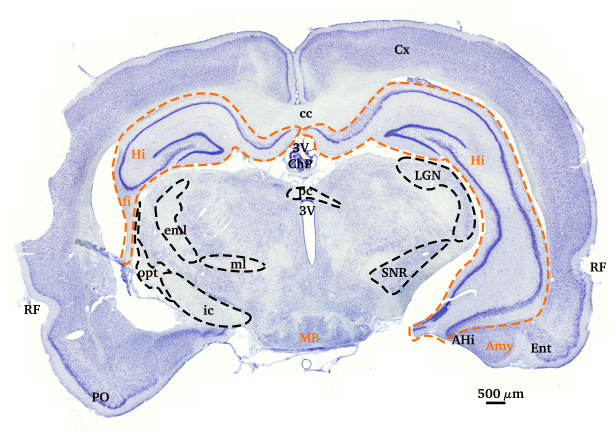
\includegraphics{pictures/Basalganglia/Hippo_uebersicht.png}
    \caption[Übersicht Hippocampus und Amygdala]{\textbf{Übersicht Hippocampus und Amygdala.} Der Hippocampus (Hi) ist innerhalb des Temporallapens an der medialen Seitenwand des lateralen Ventrikels lokalisert. Die Amygdala (Amy) liegt unterhalb des Hippocampus und ist mit ihm über die amygdaloid-hippocampale Area (AHi) verbunden. Die Fimbria (fi) bilden den Übergang zur Fornix, dem efferenten Fasertrakt des Hippocampus, der in den Mammillarkörpern (MB) des Hypothalamus endet. Außerdem in der Abbildung zu sehen: dritter Ventrikel (3V), Plexus choroideus (ChP), Corpus callosum (cc), Cortex (Cx), Lamina medullaris lateralis (eml), Entorhinaler Cortex (Ent), Capsula interna (ic), Nucleus geniculatum laterale (LGN), Leminiscus mediale (ml), optischer Trakt (opt), posteriore Kommissur (pc), primärer  olfaktorischer  Cortex (PO), Fissura rhinalis (RF), Substantia nigra pars reticularis (SNR). Nissl-Färbung (N19-4).}
    \label{fig:hippo_uebersicht}
\end{figure}

\begin{figure}[H]
    \centering
    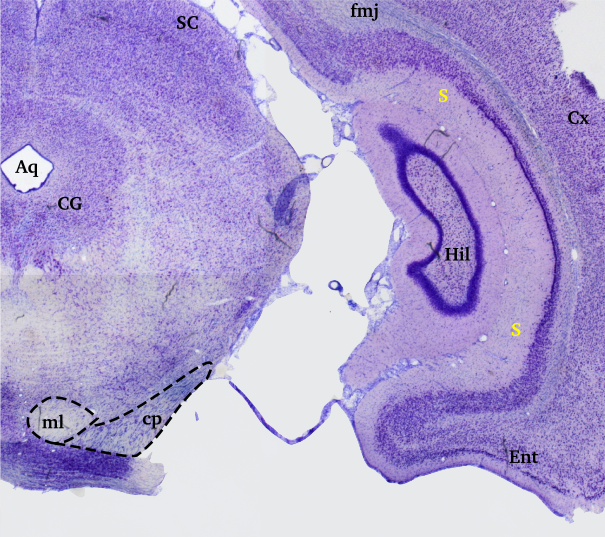
\includegraphics{pictures/Basalganglia/Subiculum.png}
    \caption[Subiculum]{\textbf{Subiculum.} Das Subiculum (S) des Hippocampus verbindet dieses mit dem Gyrus parahippocampalis. Das Hilus (Hil) bildet die dritte Zellschicht des Gyrus dentatus. Außerdem zeigt die Abbildung: 
    Aquädukt (Aq), zentrales Höhlengrau (CG), Kleinhirnpedunkle (cp), Cortex (Cx), Entorhinaler Cortex (Ent), Forceps minor des Corpus callosum (fmj), medialer Lemniscus (ml), Colliculus superior (SC). Nissl-Färbung (N14-4).}
    \label{fig:hippo_subiculum}
\end{figure}

\begin{figure}[H]
    \centering
    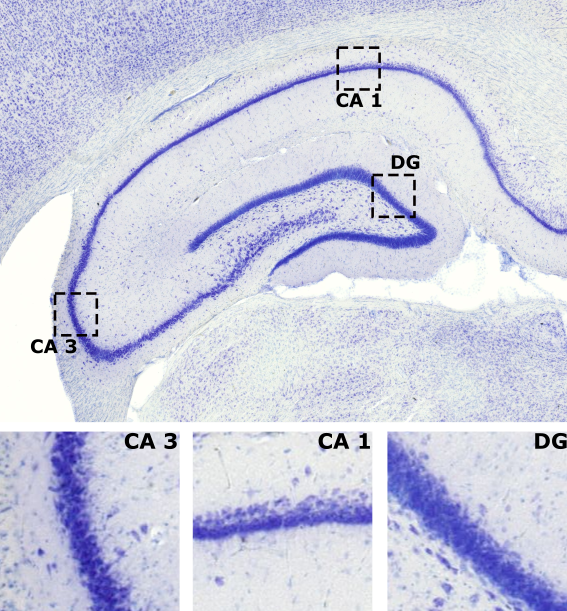
\includegraphics{pictures/Basalganglia/schichten_hippocampus.png}
    \caption[Zellschichten des Hippocampus]{\textbf{Zellschichten des Hippocampus.} Der Hippocampus besteht aus dem Gyrus dentatus (DG) und dem Ammons Horn (C1 und C3). Die markante Zellschicht (hier dunkel gefärbt und vergrößert) des Gyrus dentatus ist die Körnerschicht. Im Cornu ammonis besteht sie aus Pyramidenzellen. Dabei sind diese im Bereich des CA3 deutlich größer als in CA1. Nissl-Färbung (N19-4).}
    \label{fig:Hippocampus_zellschicht}
\end{figure}

\subsubsection*{Corpus amygdaloideum} \index{Amygdala} \index{Corpus! amygdaloideum}
Der \textbf{Corpus amygdaloideum} oder kurz \textbf{Amygdala} (altgriechisch: Mandelkern) ist innerhalb des medialen Temporallappens, rostral zum unteren Horn des lateralen Ventrikels lokalisiert (Abb.~\ref{fig:hippo_uebersicht}) \textsuperscript{\cite[Kap.~9]{trepel2011neuroanatomie}}. Funktionell lässt sich die Amygdala in drei grobe Bereiche unterteilen. Das \textbf{corticomediale Gebiet} erhält chemosensorische Afferenzen aus dem Riechhirn und die \textbf{basolateralen} und \textbf{zentralen Anteile} sind für eine emotionale Antwort und auch emotionales Lernen zuständig. Diese drei Bereiche wiederum setzen sich ungleich aus mehreren cortikalen und subcortikalen Einzelkernen zusammen. Dabei werden die Kerne des cortikalen und basolateralen Gebiets, zusammen mit den amygdalo-hippocampalen Übergang, als cortikale Regionen eingeteilt. Genauer gesagt gehören sie zum den allocortikalen Strukturen und weisen auch die typische drei-schichtige Gliederung auf. Zu den subkortikalen Zentren werden die Kerne des zentralen und medialen amygdaloiden Bereichs gezählt. Damit ist der Corpus amygdaloideum weder eine strukturelle noch funktionelle Einheit \textsuperscript{\cite[Kap.~18]{paxinos2014rat}}. \\
Die Amygdala weist ein komplexes Netzwerk an afferenten und efferenten Verbindungen auf, die die Grundlage ihrer verhaltensbezogenen Vielseitigkeit bilden. Der Input stammt dabei aus dem Thalamus, dem olfaktorischen Trakt und den Assoziationsarealen des Cortex. Außerdem erhält die Amygdala, über das mediale Vorderhirnbündel, katecholaminerge und serotonerge Fasern aus dem Hirnstamm. 
Der Großteil der efferenten Fasern verlaufen in der Stria terminalis um den Ncl. caudatus herum und enden dann im Hypothalamus des Zwischenhirns \textsuperscript{\cite[Kap.~12]{crossman2014neuroanatomy}}. Zusätzlich ziehen auch über die Fibrae amygdalofugales ventrales wichtige Faserverbindungen von der Amygdala zum frontobasalen Cortex, dem Hypothalamus oder ins Septum. Über diese Efferenzen nimmt der Corpus amygdaloideum Einfluss auf die vegetativen Bereiche des Hypothalamus. Weiterhin spielt er eine wichtige Rolle in emotional ausgelösten motorischen Verhaltensweisen, der Angstreaktion und in der Speicherung emotionaler Erinnerungen (operante oder klassische Konditionierung) \textsuperscript{\cite[Kap.~9]{trepel2011neuroanatomie}}. 

\subsubsection*{Allgemeine Funktion des limbischen Systems}
Jeder Struktur des limbischen System übernimmt eine etwas andere Aufgabe, die sich allerdings im Bereich Emotionen, Affektverhalten, Antrieb und Gedächtnis stark über-schneiden. Der Gyrus cinguli ist für den lokomotorischen Antrieb und eine vegetative Modulation zuständig. Der Gyrus parahippocampalis spielt zusammen mit dem Hippocampus eine wichtige Rolle für das explizite Gedächtnis. Des Weiteren leitet er wichtige Impulse an den Hippocampus weiter. Neben dem Gedächtnis übernimmt der Hippocampus auch eine emotionale und vegetative Funktion. Dasselbe gilt für die Amygdala, die außerdem auch verantwortlich für Affektverhalten und emotionales Lernen durch operante oder klassische Konditionierung ist. Über den Corpus mammillare schließt sich der Papez-Neuronenkreis, der die Grundlage des expliziten Gedächtnis ist. Zusätzlich ist diese Gebiet auch in Affektverhalten und vegetative Funktionen verwickelt. Damit gilt das limbische System als zentraler Entstehungsort von Gefühlen, Erinnerungen, Trieben und teilweise auch intellektueller Leistungen. Dies ist jedoch eine starke Vereinfachung, da sich diese Funktionen nicht ausschließlich auf das limbische System beschränken. Zahlreiche andere Strukturen, unter anderem der präfrontale Cortex, arbeiten zusammen mit dem limbischen System \textsuperscript{\cite[Kap.~9]{trepel2011neuroanatomie}}.    

